\subsection{Diseño Módulo 4}

En esta sección se deifine la tanto el diagrama de secuencia el cual indica la interacción del usario con el sistema, así como 
las pagínas web que se muestran en este módulo.

\subsubsection{Diagrama de secuencia}

A continuación en la \ref{fig:Sec1} se muestra el diagrama de secuencia del módulo 4, 
el cual indica la interacción del usuario con el sistema.

 \begin{figure}[htbp]
    \centering
    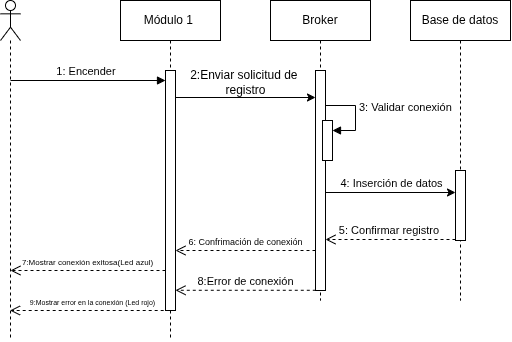
\includegraphics[width=.9\textwidth]{./UML/Modulo4/vertical1.drawio.png}
    \caption{Secuencia de interacción del usuario con el sistema en el módulo 4}
    \label{fig:Sec1}
    \end{figure} 

\subsubsection{Pantallas del usuario}

A continuación se muestran las pantallas que el usuario puede visualizar en el módulo 4, 
así como la descripción de cada una de ellas.
